\subsection{The Wave Equation}

\subsubsection{Brief Derivation}
\begin{equation} \label{eq:wave_equation}
    \frac{\partial^2 u}{\partial t^2} = c^2 \nabla^2 u = c^2 \frac{\partial^2 u}{\partial x^2}
\end{equation}

\noindent
Or in subscript notation,
\begin{equation} \label{eq:wave_equation_subscript}
    u_{tt} = c^2 u_{xx}
\end{equation}

\subsubsection{Application of the Fourier Transform}
Since \(u(x,t)\) is defined as the displacement of the wave at position \(x\) and time \(t\), we can apply the Fourier Transform to \(u(x,t)\) with respect to position \(x\) to reduce the \cref{eq:wave_equation_subscript} PDE into an ODE. Thus, let \(U(\kappa,t)\) be the Fourier Transform of \(u(x,t)\) with respect to \(x\).

\vspace{5mm}
\noindent
Taking the Fourier Transform of \cref{eq:wave_equation_subscript} with respect to \(x\),
\begin{equation}
    \mathcal{F} \left\{ u_{tt} \right\} = \mathcal{F} \left\{ \alpha^2 u_{xx} \right\}
\end{equation}

\noindent
Using \cref{fourier_scaling},
\begin{equation}
    \mathcal{F} \left\{ u_{tt} \right\} = \alpha^2 \mathcal{F} \left\{ u_{xx} \right\}
\end{equation}

\noindent
Using \cref{fourier_derivative},
\begin{align}
    \mathcal{F} \left\{ \frac{\partial^2 u(x, t)}{\partial x^2} \right\} & = i \kappa \mathcal{F} \left\{ \frac{\partial u(x, t)}{\partial x} \right\} \\
    & = -\kappa^2 \mathcal{F}\{ u(x, t) \} \\
    & = -\kappa^2 U
\end{align}

\noindent
Therefore,
\begin{align}
    \mathcal{F} \left\{ u_{tt} \right\} &= -\alpha^2 \kappa^2 U \\
    \frac{d^2 U}{dt^2} &= -c^2 \kappa^2 U \label{eq:wave_equation_fourier}
\end{align}

\subsubsection{Boundary Conditions} % TODO: Add boundary conditions to the heat equation.

\subsubsection{Numerical Solution to Wave Equation}
\cref{eq:wave_equation_fourier} is a decoupled ODE that can be easily numerically integrated. A numerical solution to \cref{eq:wave_equation_fourier} using a fifth-order Runge-Kutta approximation in Python is presented below:

\begin{figure}[H]
    \centering
    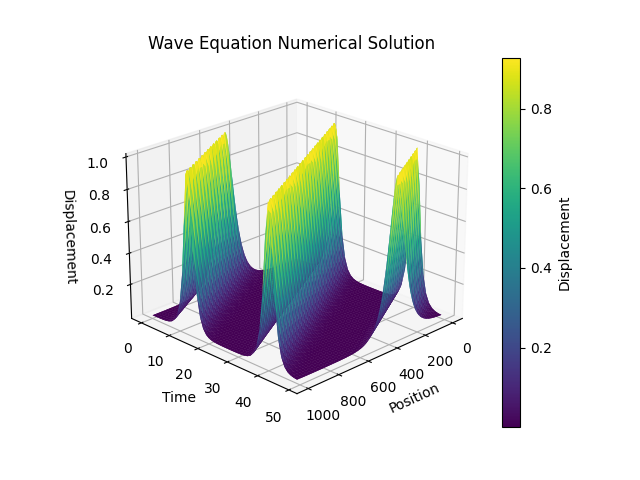
\includegraphics[width=110mm,height=\textheight,keepaspectratio]{images/wave_equation_numerical.png}
    \caption{Defining the initial wave displacement \(u(x, 0)=\sech(x)\), this plot shows the temperature change along \(x\) and \(t\) by performing a numerical integration of \cref{eq:wave_equation_fourier}.}
    \label{fig:wave_equation_numerical}
\end{figure}

% \subsubsection{Analytical Solution to Wave Equation} 
% This is a maybe section. Possibly replace this section with a section on the applicability of the Fourier Transform to reduce PDEs to ODEs...?